\documentclass[windows,csize4]{BHCexam}
%\documentclass[windows,csize4,answers]{BHCexam}

\usepackage{multicol} % 分栏
\usepackage{polynom} % 多项式除法
\pagestyle{fancy}
\fancyfoot[C]{\kaishu \small 第 \thepage 页 共 \pageref{lastpage} 页}
%\fancyhead[L]{\includegraphics[width=2cm]{qrcode.png}}
\title{声音}
%\subtitle{数学文科试卷}
%\notice{满分150分, 120分钟完成, \\	允许使用计算器,答案一律写在答题纸上.}
%\author{Gavin Chen}
%\date{\today}
\usepackage{enumerate} % 编号
\usepackage{cases}
\usepackage{subfigure}
\usepackage{graphicx}

\begin{document}

\maketitle

\begin{groups}
    \group{声音的产生与传播}{}
    声音是如何产生的?
    \begin{itemize}
        \item 由物体振动产生。振动停止,声音停止。
        \item 声源:正在发声的物体。
        \item 固体、液体、气体都可以振动产生声音。
    \end{itemize}

    声音是如何传播的?
    \begin{itemize}
        \item 声音传播需要介质。例子:把闹钟放在密封空间抽空气,声音越来越轻。(真空不能传递声音)
        \item 声音在不同介质中的传播速度,一般来说,传播速度固体>液体>气体。
        \item 声音以波的形式传播,称之为声波。
    \end{itemize}

    人耳听到声音,通常是由空气传播,然后进入耳道。但是也可以用骨传导耳机。(据说贝多芬耳朵聋了之后就采用类似方法作曲)

    想一想,如果声源在移动,会不会影响声音传播的速度?比如救护车疾驶而过,这个时候声音通过空气传播,那么救护车的速度会不会影响它发出的警报声在空气中的传播速度呢?
    
    \group{声音的特征}{}

    人耳感觉到的声音的强弱程度叫做响度。想一想,下图中两个声波,那个更响?
    图 \ref{fig:fig_2_1}声波的形状和响度
    \begin{figure}[htb]
        \centering
        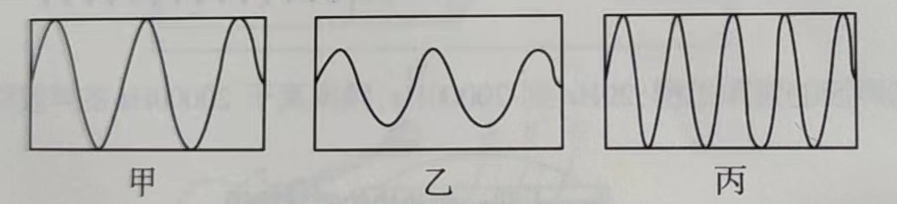
\includegraphics [scale=0.75,trim=0 0 0 0]{./image/fig_2_1.PNG}
        \caption{声波的形状和响度} 
        \label{fig:fig_2_1}
    \end{figure}

    影响响度的因素
    \begin{itemize}
        \item 响度和振幅有关,振幅越大,响度越大。
        \item 响度和接收者离开声源的距离有关,距离越近,响度越大。
        \item 利用喇叭,可以是声波的传播方向更加集中,可以在不改变距离和声源振幅的情况下增加响度及传播更远的距离。
    \end{itemize}

音调:声音的高低。有时也叫做音高。比如常说的男高音,女中音就是指的音调。

\begin{itemize}
    \item 音调和发声体振动的快慢(即频率)有关。
    \item 频率:物体每秒钟振动的次数,单位:次/秒。即赫兹(Hz)
    \item 频率的物理意义:反映物体振动快慢。
    \item 频率低,音调低
\end{itemize}

回到图 \ref{fig:fig_2_1}中,甲和丙什么一样,什么不一样?
回到刚才救护车的例子,声音传播的速度没变,但是什么变了?

图 \ref{fig:fig_2_2}声音的频率,数一下下面两者的频率分别是多少?
\begin{figure}[htb]
    \centering
    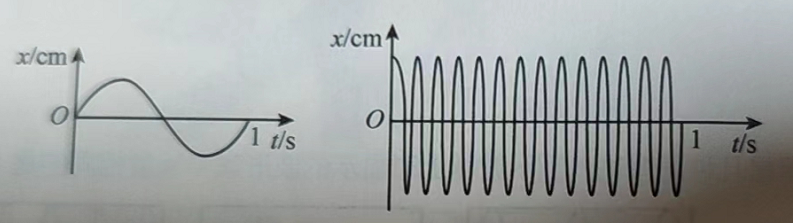
\includegraphics [scale=0.75,trim=0 0 0 0]{./image/fig_2_2.PNG}
    \caption{声音的频率} 
    \label{fig:fig_2_2}
\end{figure}

小知识,人耳的听觉范围$20Hz~20000Hz$,常见动物的听力和发声频率,见图 \ref{fig:fig_2_3}.
\begin{figure}[htb]
    \centering
    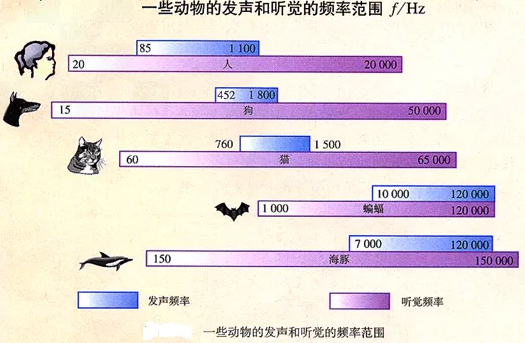
\includegraphics [scale=0.75,trim=0 0 0 0]{./image/fig_2_3.PNG}
    \caption{声音的频率} 
    \label{fig:fig_2_3}
\end{figure}

小知识,对弦乐类乐器,其音调和弦的粗细、长短、松紧程度有关系。弦越短,越细,越紧,那么音调就越高;对管乐类乐器,一般其空气柱长度越短,音调越高。

音色,声音的特色,是我们分辨各种声音的依据。比如钢琴和小提琴的音色不一样。
\begin{itemize}
    \item 发声体本身的材料、结构是影响音色的主要因素。
    \item 发声体发出的声音一般不是单一的频率,而是各个频率声波的组合。频率的组合情况不同,音色就不同。
\end{itemize}

\begin{figure}[htb]
    \centering
    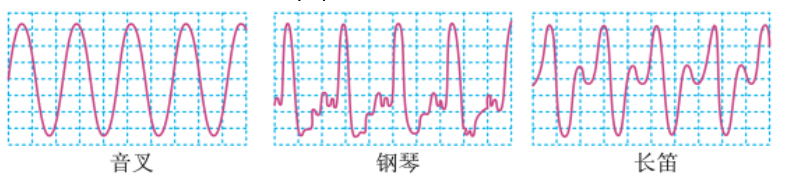
\includegraphics [scale=0.75,trim=0 0 0 0]{./image/fig_2_4.PNG}
    \caption{音叉,钢琴和长笛的音色} 
    \label{fig:fig_2_4}
\end{figure}
想一想,图\ref{fig:fig_2_4}中,响度一样嘛?音调一样嘛?音色一样嘛?



噪音和乐音
\begin{itemize}
    \item 环境学中,把对人们休息,工作,学习产生干扰的声音叫噪音。
    \item 物理学中,把声体无规则振动发出的声音叫噪音。小知识:宇宙背景辐射。
\end{itemize}
噪声的单位:分贝(dB)。 0dB是人们刚能听到的最微弱的声音。
\begin{figure}[htb]
    \centering
    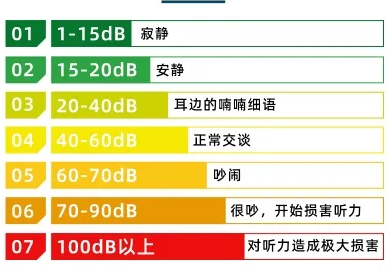
\includegraphics [scale=0.75,trim=0 0 0 0]{./image/fig_2_5.PNG}
    \caption{常见声音的大小} 
    \label{fig:fig_2_5}
\end{figure}
想一想,如何减弱噪音?
\begin{itemize}
    \item 声源处:加消音器,禁止鸣笛
    \item 传播过程中:隔音墙,绿化
    \item 人耳处:噪音耳塞
\end{itemize}
乐音:悠扬悦耳,令人心旷神怡的声音。

    \group{如何利用声音}{}
    声音技能传递信息,也能传递能量。
    \begin{itemize}
        \item 声音传递信息:超声检查,回声定位
        \item 声音传播能量:超声碎石,超声清洁玻璃
    \end{itemize}

\end{groups}

\begin{groups}
%例题开始

\end{groups}

\label{lastpage}
\end{document}